
\section{KIDs specific systematics and application to CMB polarization}

\begin{itemize}
\item glitch (because it's important in a space oriented discussion)
\item non linearity. Explain frequency modulation, RF and PF reconstructions
  that may not be strictly linear
\item Explain what we mean by non linearity (ref to previous papers that showed
  the linearity of the KIDs response and that we look at the next order
  correction). Polarized equations with the non linear term.
\item Describe the simulation method : on simule une planete scannee a une
  certaine vitesse, on recalcule le flux etc... pour mesurer la
  non-lin\'earit\'e.
\item Results in RF and PF
\item Application to CMB maps and power spectra estimation
\item HWP associated systematics. The modulation of the HWPSS may bias the
  measurement by inducing non linearity.
\end{itemize}

In view of future utilizations of KIDs in space mission it is necessary to demonstrate the capabilities and the suitability of KIDs arrays in a space like environment. In this section we will adress some of the systematics effects that need to be taken into account during the design of futur generation detector arrays for space applications, such as the KIDs non-linearity.\\

\subsection{Cosmic rays impact on KIDs array}

One of the major problems for space based missions is the impact of an intense flux of high energy particles, referred to as Cosmic Rays (CR) on the detectors. Primary CR are produced by the Sun and by other galactic sources. They are mostly composed by protons (90\%), helium nuclei (9\%) and a few heavier nuclei and electrons (1\%). The CR spectrum is peaked aroud 200 MeV, thus the particles have sufficient energy to penetrate the detectors and give an unwanted signal. The Planck satellite \citep{2014A&A...571A..10P} has demonstrated that the impact of CR on the detectors are a key problem for space missions. Indeed, the glitches caused by CR can mask the real data and induce a loss of an important fraction of it.\\
Experiments have been done to construct a setup that allows to study the behavior of KIDs arrays under typical conditions of a space-borne observatory, and establish the compatibility of KIDs with a space environment \citep{2016A&A...592A..26C,2016SPIE.9914E..0NM}. When the detector is hit by a CR there is a lapse of time during which the sensor is 'blind' to the incoming scientific data. The length of this dead-time depends on the response time of the KID (time constant) which is determined by the quasi particle lifetime. \citet{2012ApPhL.100w2601M} have shown for KID, this time constant is equal to about tens of microseconds which is faster than bolometers (from 5-10 ms to 2s). This means that for the same CR hit, less data is lost when using KIDs arrays. Plus, the experiments have confirmed the fact that KID recover their initial state in less than 5 milliseconds. Finally, \citet{2016SPIE.9914E..0NM} concluded that the percent level of data loss per pixel by a KIDs array placed in a space environment is about 1 \% compared to 15 \% for Planck HFI bolometers.\\ Compared to bolometers, the KID technology shows promising results for compatibility with a space-borne mission, as their extremely short glitch time constant permits to greatly reduce the data loss fraction due to CR impacts. 

\subsection{KIDs non-linearity}

One of the key systematic effect that we must take into account is the KID non-linearity induced by the detector and the method we use to reconstruct the absorbed signal. In this paper, we will focus on the KID non linearity and how it impacts on a measurement of the CMB polarization.\\

The KIDs linearity has been demonstrated, over a large power range, in laboratory under realistic conditions as shown in Fig. \ref{KID-lin}. As we can see, at 300K the response of the KID is still under a linear regime.

\begin{figure}[h]
\center
	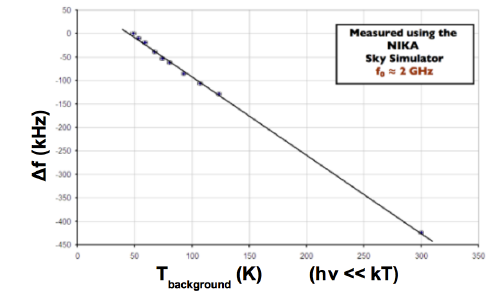
\includegraphics[scale=0.4]{KID-linearity-Monfardini2014.png}
	\caption{KID linarity demonstrated in laboratory under realistic conditions. Y-axis : frequency shift of the resonance (KID measured signal), X-axis : optical background temperature. The solid line represents the linear fit of the experimental points. Credits : \citet{2014JLTP..176..787M}.}
	\label{KID-lin}
\end{figure}

In this section we look at the next order correction, meaning that we will focus on the non-linear term produced by the detector and the way that we reconstruct the signal. A measure done by the KID is defined by $m = T + P$, with $T$ and $P$ representing the temperature and polarization. The non-linearity is characterized  by the $\varepsilon$ coefficient in $ m = m_{1} + \varepsilon m_{1}^{2}$. We have : 

\begin{equation}
\begin{split}
m & = m_{1} +\varepsilon' (T+P)^{2} \\
 & = T + P + \varepsilon'(T^{2} + P^{2} + 2TP) 
\end{split}
\end{equation}

Therefore, knowing that $T=I$ and $P = Q\cos(2\alpha) + U \sin(2\alpha)$, the polarized equation with a non-linear term is given Eq. \ref{eq-NL}.

\begin{equation}
m  \simeq (I + \varepsilon' I^{2}) + (Q + 2\varepsilon' IQ) \cos(2\alpha) + (U + 2 \varepsilon' IU) \sin(2\alpha)
\label{eq-NL}
\end{equation}

The non-linear coefficient is induced by the detector and the method used to reconstruct the signal. These methods are described in the following section.



\subsection{Application to CMB maps and power spectra estimations}
\subsection{HWP associated systematics}
